\begin{figure}[tb]
\centering
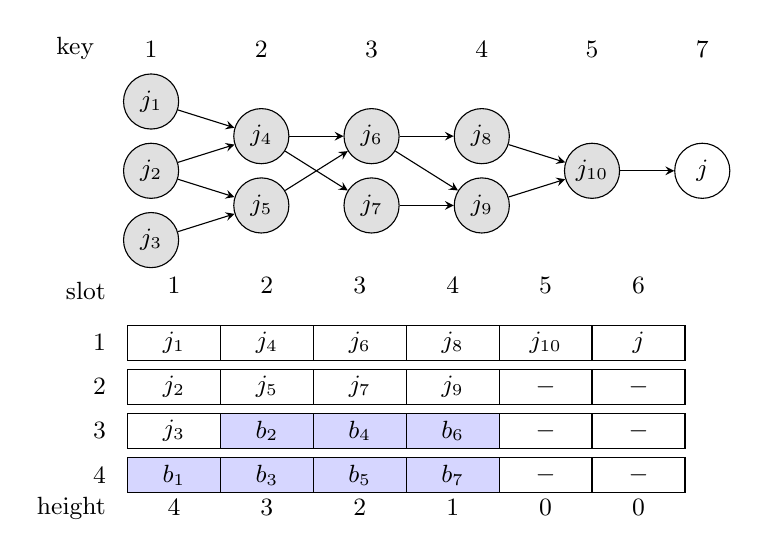
\begin{tikzpicture}[x=1cm,y=.8cm,>=stealth,font=\small,
  job/.style={circle,draw,fill=black!12,minimum size=7mm,inner sep=0pt},
  target/.style={circle,draw,minimum size=7mm,inner sep=0pt}]
  % The early-ancestor DAG. Numbers above columns are priority keys.
  \node[job] (a) at (.3,1.1) {$j_1$};
  \node[job] (b) at (.3,0) {$j_2$};
  \node[job] (c) at (.3,-1.1) {$j_3$};
  \node[job] (d) at (1.7,.55) {$j_4$};
  \node[job] (e) at (1.7,-.55) {$j_5$};
  \node[job] (f) at (3.1,.55) {$j_6$};
  \node[job] (g) at (3.1,-.55) {$j_7$};
  \node[job] (h) at (4.5,.55) {$j_8$};
  \node[job] (i) at (4.5,-.55) {$j_9$};
  \node[job] (k) at (5.9,0) {$j_{10}$};
  \node[target] (j) at (7.3,0) {$j$};
  \foreach \from/\to in {a/d,b/d,b/e,c/e,d/f,e/f,d/g,f/h,f/i,g/i,h/k,i/k,k/j}
    \draw[->] (\from)--(\to);
  \foreach \x/\key in {.3/1,1.7/2,3.1/3,4.5/4,5.9/5,7.3/7}
    \node[above] at (\x,1.65) {$\key$};
  \node[anchor=east] at (-.3,1.95) {key};
  % Rows are machines and columns are slots.
  \foreach \x/\slot in {0/1,1.18/2,2.36/3,3.54/4,4.72/5,5.90/6}
    \node[above] at (\x+.59,-2.1) {$\slot$};
  \node[anchor=east] at (-.15,-1.9) {slot};
  \foreach \y/\machine in {-2.45/1,-3.15/2,-3.85/3,-4.55/4}
    \node[anchor=east] at (-.15,\y-.28) {$\machine$};
  \node[anchor=east] at (-.15,-5.35) {height};
  \foreach \x/\one/\two/\three/\four in {
    0/j_1/j_2/j_3/b_1,
    1.18/j_4/j_5/b_2/b_3,
    2.36/j_6/j_7/b_4/b_5,
    3.54/j_8/j_9/b_6/b_7,
    4.72/j_{10}/{-}/{-}/{-},
    5.90/j/{-}/{-}/{-}}
  {
    \foreach \y/\entry in {-2.45/\one,-3.15/\two,-3.85/\three,-4.55/\four}
    {
      \draw (\x,\y) rectangle ++(1.18,-.56);
      \node at (\x+.59,\y-.28) {$\entry$};
    }
  }
  \foreach \x/\y/\entry in {
    0/-4.55/b_1,1.18/-3.85/b_2,1.18/-4.55/b_3,
    2.36/-3.85/b_4,2.36/-4.55/b_5,
    3.54/-3.85/b_6,3.54/-4.55/b_7}
  {
    \fill[blue!16] (\x,\y) rectangle ++(1.18,-.56);
    \draw (\x,\y) rectangle ++(1.18,-.56);
    \node at (\x+.59,\y-.28) {$\entry$};
  }
  \foreach \x/\height in {0/4,1.18/3,2.36/2,3.54/1,4.72/0,5.90/0}
    \node at (\x+.59,-5.35) {$\height$};
\end{tikzpicture}
\caption{A priority-band example with four machines. The graph shows the
predecessors of the target $j$ and their precedence arcs. The number
above each column is the priority key. The seven independent jobs
$b_1,\ldots,b_7$ have depth one and key $6$. The jobs are numbered in the
order $j_1,\ldots,j_{10},j,b_1,\ldots,b_7$. With threshold $5.9$, the
$b_i$ lie in the priority band $(5.9,7]$. The table gives a non-delay priority schedule.
Each of its first four slots is full and contains a band job. Its final row
shows the height of the unfinished early-key predecessors after each slot,
starting from height five. The band slots force this height to fall to one
even though no machine is idle. Dashes denote idle machines.}
\label{fig:band-progress}
\end{figure}
